\documentclass{article}
\usepackage{graphicx} % Required for inserting images
\usepackage{kotex}
\usepackage{amsmath,amssymb}
\usepackage{booktabs,multirow}
\usepackage[margin=2.2cm]{geometry}
\usepackage{caption}
\captionsetup{font=small,labelfont=bf}

\title{[Conference\_IWAIT27] 전기헌\\[4pt]
\large 저프레임률 이중 각도 IR-UWB 레이더와 단계형 캘리브레이션을 결합한 확산 트랜스포머 기반 보행 중 호흡 파형 복원 및 실내 위치 추정}
\author{KW.HAI\_Lab}
\date{October 2026}

\begin{document}

\maketitle

\begin{abstract}
비접촉 레이더 호흡 측정 연구의 대부분은 사람이 레이더 정면에 정지해 있고 높은 프레임률(약 50~fps)로 위상을 추적할 수 있는 상황을 가정한다.
그러나 실내 공간을 이동하는 사람을 저가 IR-UWB 레이더(17~fps)로 측정하면 보행에 따른 몸통 변위가 프레임 간 위상 변화 한계를 넘어서기 때문에,
위상 기반 복조로는 호흡 파형을 직접 얻을 수 없다. 본 논문은 이 문제를 (i) 두 대의 레이더를 ㄱ자 경로에 서로 다른 각도로 배치하여 어느 위치에서든 한 대는
몸의 정면 또는 후면을 관측하도록 하는 배치, (ii) 레이더에서 얻은 개인별 호흡수 단서와 코스 리듬 사전정보, 짧은 벨트 등록을 단계적으로 결합하는 캘리브레이션,
(iii) 이들 조건을 받아 연속 호흡 파형과 14개 구역 위치를 함께 출력하는 조건부 확산 트랜스포머(DiT)로 해결한다.
피험자 40명의 보행 데이터에 대해 피험자 단위 5-fold 교차검증으로 평가한 결과, 벨트 없이 레이더만으로 캘리브레이션한 경우 호흡수 오차가 2.17에서 1.64~bpm으로 줄고
숨 봉우리 $\pm$0.5~s 일치율이 38.2\%에서 41.6\%로 증가하였다. 보행 1바퀴(42~s)의 벨트 등록을 더하면 호흡수 오차 0.97~bpm, 봉우리 일치율 42.5\%로 84~s 등록과 동등한 성능을 보였다.
동일한 데이터와 캘리브레이션 조건에서 TCN, U-Net, IQ-VED, 트랜스포머 회귀 모델, RF-Carer보다 숨 타이밍이 3.5~6.4\%p 높았고, 42~s 등록 조건에서는 호흡수 오차도 0.44~0.59~bpm 낮았다.
위치 추정은 14개 구역에서 92.9\%의 정확도를 보였다.
\end{abstract}

\noindent\textbf{Keywords:} IR-UWB radar, respiration reconstruction, diffusion transformer, calibration, indoor localization, walking

%==============================================================
\section{서론}
%==============================================================
호흡은 수면, 스트레스, 심폐 질환 상태를 반영하는 핵심 생체 신호이며, 일상 공간에서 장비를 착용하지 않고 지속적으로 측정하려는 수요가 커지고 있다.
IR-UWB 레이더는 조명과 사생활 문제에서 자유롭고 저가·저전력으로 구현할 수 있어 비접촉 호흡 측정 수단으로 주목받아 왔다.
그러나 기존 연구의 대부분은 사람이 레이더 정면에 앉거나 누워 정지한 상황을 다루며, 움직임이 있는 경우에도 높은 프레임률에서 위상을 연속 추적하는 것을 전제로 한다.

실제 생활 공간에서는 사람이 이동하고, 레이더에 대한 방향이 계속 바뀌며, 저가 장치는 프레임률이 낮다.
본 연구에서 사용한 레이더는 17~fps로 동작하며 반송파 7.29~GHz에서 프레임당 위상이 $\lambda/4$ 이내로 변하려면 반경 방향 속도가 0.175~m/s 이하여야 한다.
보행 중에는 이 조건이 자주 깨져, 6~s 길이 구간에서 위상이 일관되게 유지되는 비율이 정지 대기 시 83\%에서 보행 시 0.3\%로 떨어졌다.
즉 \textbf{17~fps 보행 조건에서는 위상 복조로 호흡 파형을 직접 얻을 수 없으며}, 호흡 정보는 주로 몸이 잠시 멈추는 순간의 진폭 변화에 남는다.

이에 본 논문은 신호 자체에서 파형을 복조하는 대신, 레이더가 제공하는 부분적인 정보와 사람별·환경별 사전정보를 결합해 호흡 파형을 \textit{복원}하는 접근을 제안한다.
주요 기여는 다음과 같다.
\begin{itemize}
  \item \textbf{이중 각도 배치}: 두 대의 IR-UWB 레이더를 ㄱ자 경로의 서로 수직한 두 팔 방향에 배치하여, 경로의 93\% 지점에서 적어도 한 대가 몸의 정면 또는 후면을 관측하도록 하였다.
  \item \textbf{단계형 캘리브레이션}: 벨트 없이 레이더 단서로 개인 호흡수를 추정하는 단계, 코스 리듬 사전정보를 더하는 단계, 필요 시 보행 1바퀴(42~s)의 짧은 벨트 등록을 더하는 단계를 정의하고 각 단계의 기여를 정량화하였다.
  \item \textbf{다중 작업 조건부 확산 트랜스포머}: 두 레이더의 신호와 기하 정보를 조건으로 연속 호흡 파형과 14개 구역 위치를 함께 출력하며, 캘리브레이션 정보를 샘플링 단계의 조건으로 받아 재학습 없이 개인화한다.
  \item 피험자 40명, 5종의 회귀 기반 비교 모델, 동일한 캘리브레이션 조건에서의 비교와 시간 이동 대조 실험을 통해 레이더가 기여하는 정보(숨 타이밍)와 캘리브레이션이 결정하는 정보(호흡수 수준)를 분리하여 보고한다.
\end{itemize}

%==============================================================
\section{시스템 및 데이터}
%==============================================================
\subsection{측정 환경과 레이더 배치}
그림~\ref{fig:layout}과 같이 실내에 14개 구역(각 약 0.47$\times$0.40~m)으로 이루어진 ㄱ자 보행 경로를 구성하였다.
피험자는 구역마다 약 3~s씩 머물며 경로를 따라 이동하여 한 바퀴(42~s)를 반복한다.
레이더 두 대(COM, TV)는 각각 경로의 세로 팔과 가로 팔 방향을 바라보도록 설치하였다.
이 배치에서는 경로의 진행 방향을 기준으로 어느 지점에서든 한 대는 몸의 정면 또는 후면을, 다른 한 대는 측면을 관측한다(그림~\ref{fig:layout} 가운데).
정면·후면 관측($|\cos\theta|>0.7$) 비율은 레이더별로 약 50\%이지만 두 대를 합치면 93\%에 이른다.
레이더는 Novelda X4 기반 IR-UWB 장치(대역 6.6--7.8~GHz, 반송파 7.29~GHz, 17~fps, 거리 해상도 bin 0.0514~m)이다.

\begin{figure}[t]
  \centering
  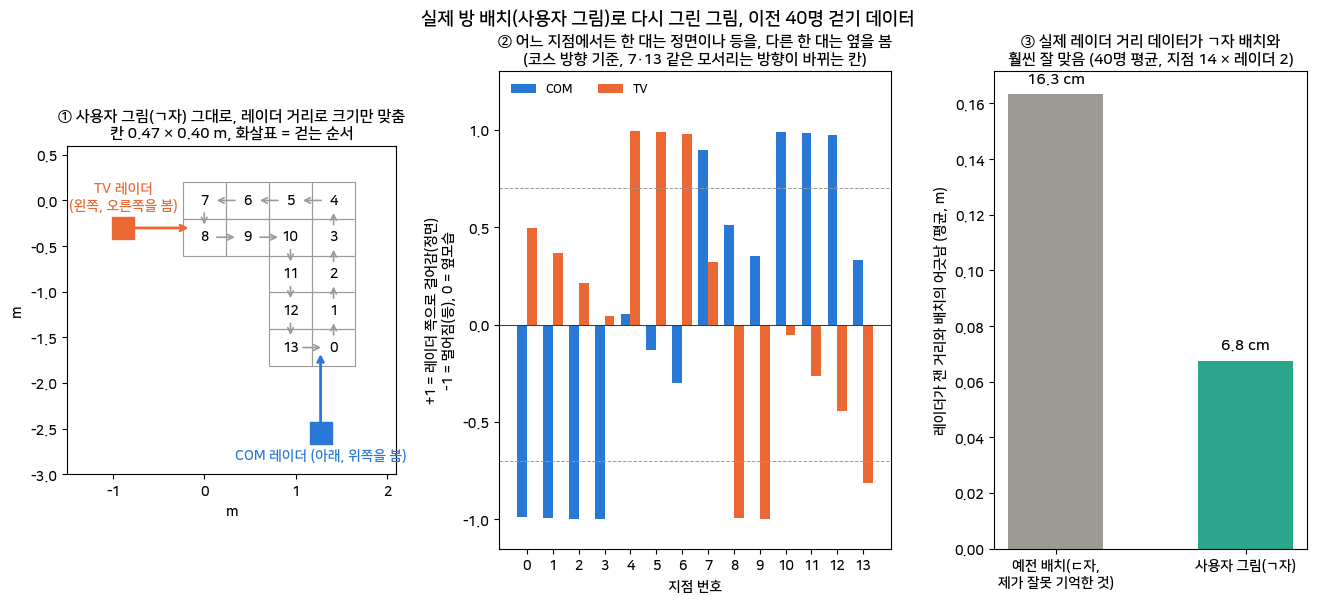
\includegraphics[width=\linewidth]{layout_L.png}
  \caption{ㄱ자 보행 경로와 두 레이더의 배치. (왼쪽) 14개 구역과 보행 순서, 레이더 위치. (가운데) 각 구역에서 진행 방향과 레이더 시선 사이의 각도 코사인; 한 대가 정면·후면($\pm1$)을 볼 때 다른 한 대는 측면(0 근처)을 본다. (오른쪽) 측정된 레이더 거리와 배치 모델의 평균 오차.}
  \label{fig:layout}
\end{figure}

\subsection{데이터}
성인 피험자 40명이 경로를 반복 보행하는 동안 두 레이더 신호와 BIOPAC 호흡 벨트 신호를 동기 기록하였다(1인당 약 4~분).
벨트 신호의 숨 봉우리와 골은 수동 검수를 거쳐 기준값으로 사용하였다.
기록의 처음 84~s는 캘리브레이션 구간으로 두고, 평가는 그 이후 구간(초기 과도 구간 12~s 제외, 96~s부터 기록 끝까지)에서 수행하였다.

%==============================================================
\section{제안 방법}
%==============================================================
\subsection{신호 전처리}
원시 레이더 프레임에서 배경을 제거한 뒤 거리-시간 영상에서 몸통 bin을 추적한다.
레이더마다 직접 경로(LOS)와 다중 경로 후보 bin을 정하고, 각 후보의 진폭 포락선과 프레임 간 위상 증분을 3~s 단위 청크로 나누어 모델 입력으로 사용한다.
추가로 레이더별 거리·속도, 직접/다중 경로 진폭비 등 기하 문맥과 거리 프로파일을 조건으로 함께 제공한다.

\subsection{다중 작업 조건부 확산 트랜스포머}
42~s 창을 3~s 길이의 14개 토큰으로 나누고, 각 토큰에 해당 청크의 레이더 조건을 부여한다.
토큰 사이 self-attention으로 창 전체의 레이더 정보를 통합하며, 조건은 adaLN 변조로 주입한다.
학습은 DDPM 목적함수(잡음 예측 MSE)에 14개 구역 분류 손실을 더해 수행하고, 추론은 DDIM 50단계로 수행한다.
연속 기록은 6~s씩 겹치는 창을 이어 생성하되, 겹치는 부분을 직전 출력으로 고정하고 나머지를 생성하는 이어 그리기(RePaint 방식) 샘플링으로 이음매 없이 만든다.
모델 크기는 4.25~M 파라미터이며, 42~s 창 하나를 생성하는 데 CPU 1스레드에서 0.29~s, GPU(RTX A6000)에서 0.44~s가 걸린다(실시간 대비 0.008배).

\subsection{단계형 캘리브레이션}
보행 중 레이더 스펙트럼만으로는 개인의 호흡수를 안정적으로 추정하기 어렵다. 이를 보완하기 위해 다음 세 단계를 정의한다.

\paragraph{(1) 레이더 기반 호흡수 앵커.}
벨트 없이 레이더에서 얻은 사람 단위 단서 세 가지, 즉 보행 중 TV 위상 증분의 흔들림(J), 코스 위치별 평균 대비 TV 진폭 변동(T), 보행 시작 전 정지 대기 구간에서 두 레이더 진폭의 자기상관으로 잰 호흡수(W)를
다른 피험자들의 벨트 호흡수에 회귀하여(leave-one-subject-out) 대상자의 호흡수 앵커를 얻는다.
앵커는 DDIM 샘플링의 각 단계에서 앵커 주변 좁은 대역으로 스펙트럼을 당기는 guidance로 적용되며, 앞쪽 25단계는 강하게($g{=}1.0$), 뒤쪽 25단계는 약하게($g{=}0.2$) 적용한다.

\paragraph{(2) 코스 리듬 사전정보.}
보행 중 호흡은 3~s 구역 전환 리듬에 위상이 맞춰지는 경향이 있다. 학습 fold 피험자들의 벨트에서 구역 주기 안의 평균 숨 위상을 구해 템플릿으로 만들고,
대상자의 앵커가 20$\pm$2~bpm 범위일 때 샘플링 과정에 섞어 넣는다. 대상자 본인의 벨트는 사용하지 않는다.

\paragraph{(3) 짧은 벨트 등록(선택).}
보행 1바퀴(42~s) 동안만 벨트를 착용하여, 숨 개수로 호흡수 앵커를 정하고, 그 구간으로 모델을 짧게 미세조정(few-shot)하며, 등록 구간 끝의 벨트 파형을 생성의 시작점으로 사용한다.

%==============================================================
\section{실험 설정}
%==============================================================
\textbf{평가 방식.} 피험자 단위 5-fold 교차검증을 사용하여 평가 대상자는 학습에 포함되지 않는다. 가중치 시드 3개의 결과를 피험자별로 평균한 뒤 40명 평균을 보고하며, 유의성은 피험자 단위 짝지은 Wilcoxon 검정으로 판단하였다.

\textbf{지표.} (i) 호흡수 오차: 출력과 벨트의 숨 개수로 구한 분당 호흡수 차이의 절댓값, (ii) 숨 봉우리 및 골 일치율: 검수된 벨트 봉우리(골) 중 $\pm$0.5~s 안에 출력 봉우리(골)가 있는 비율.
(iii) 우연 대비 타이밍: 출력을 10--30~s 원형 이동했을 때의 봉우리 일치율을 우연 수준으로 보고 그 차이를 함께 보고한다.

\textbf{비교 모델.} 동일한 입력과 fold로 학습한 TCN, U-Net, IQ-VED, 트랜스포머 회귀 모델(DiT와 같은 토큰 구조), RF-Carer를 비교하였다.
회귀 모델에는 동일한 호흡수 앵커를 출력의 좁은 대역 투영으로 적용하고($g{=}1$), 벨트 등록 조건에서는 동일한 42~s 벨트로 미세조정과 앵커를 함께 적용하였다.

%==============================================================
\section{결과}
%==============================================================
\subsection{캘리브레이션 단계별 성능}
표~\ref{tab:tier}는 캘리브레이션 단계별 DiT의 성능이다.
레이더만으로 캘리브레이션한 경우 캘리브레이션 없음 대비 호흡수 오차가 0.54~bpm 감소하고($p{=}.037$) 봉우리 일치율이 3.4\%p 증가하였다($p{=}.034$).
우연 대비 타이밍은 캘리브레이션 없이는 +2.1\%p로 유의하지 않았으나, 레이더 캘리브레이션 후 +5.7\%p($p{=}.001$), 42~s 등록 후 +7.2\%p($p<10^{-4}$)로 커졌다.
같은 호흡수의 사인파와 비교하면 레이더 캘리브레이션 출력의 봉우리 일치율이 8.1\%p 높아($p{=}.004$), 타이밍이 호흡수 앵커만으로 얻어지는 것이 아님을 보여 준다.
42~s 등록은 84~s 등록과 동등한 성능(0.97 대 1.01~bpm)을 보여, 캘리브레이션에 필요한 벨트 착용 시간을 절반으로 줄일 수 있었다.

\begin{table}[t]
\centering
\caption{캘리브레이션 단계별 DiT 성능(40명, 3시드, 96~s부터). 괄호는 fold 간 표준편차.}
\label{tab:tier}
\begin{tabular}{lccccc}
\toprule
캘리브레이션 & 벨트 사용 & 호흡수 오차 (bpm) & 봉우리 (\%) & 골 (\%) & 우연 대비 (\%p) \\
\midrule
없음 & -- & 2.17 (0.69) & 38.2 & 38.4 & +2.1 \\
레이더 기반 (제안) & -- & 1.64 (0.33) & 41.6 & 41.3 & +5.7 \\
레이더 + 42~s 벨트 등록 & 42~s & \textbf{0.97} (0.29) & \textbf{42.5} & \textbf{42.3} & \textbf{+7.2} \\
\midrule
참고: 84~s 벨트 등록 & 84~s & 1.01 (0.28) & 42.5 & 42.2 & +6.4 \\
참고: 레이더 앵커 호흡수 사인파 & -- & 1.66 & 33.6 & 33.7 & $-2.5$ \\
\bottomrule
\end{tabular}
\end{table}

레이더 기반 캘리브레이션에서 오차가 큰 피험자는 대부분 호흡수가 집단 평균(약 21.7~bpm)에서 멀리 떨어진 사람이었다.
사후 분석으로, 오차가 가장 큰 5명(12.5\%)에게만 42~s 등록을 적용하면 전체 호흡수 오차는 1.64에서 1.26~bpm으로 줄었다.
이는 소수의 사람에게만 짧은 등록을 추가해도 집단 전체 성능을 크게 개선할 수 있음을 시사한다.

\subsection{비교 모델과의 비교}
표~\ref{tab:base}와 그림~\ref{fig:compare}는 같은 데이터, 같은 fold, 같은 채점 방식에서의 비교 결과이다.
캘리브레이션이 없을 때는 모든 모델의 성능이 비슷하였다.
레이더 기반 캘리브레이션에서는 모든 모델이 같은 앵커를 받으므로 호흡수 오차가 거의 같았지만(1.62--1.69~bpm), 숨 봉우리 일치율은 DiT가 3.2--5.1\%p 높았다.
42~s 벨트 등록 조건에서는 DiT가 호흡수 오차(0.97 대 1.41--1.56~bpm, 모든 비교 $p<.05$)와 봉우리 일치율(+3.5--6.4\%p) 모두에서 앞섰다.
그림~\ref{fig:tradeoff}는 같은 레이더 앵커를 줄 때 회귀 모델은 호흡수만 앵커에 맞춰지고 봉우리 일치율은 거의 변하지 않는 반면, DiT는 두 지표가 함께 개선됨을 보여 준다.

\begin{table}[t]
\centering
\caption{비교 모델과의 성능 비교: 호흡수 오차 (bpm) / 숨 봉우리 일치율 (\%). 40명, 3시드, 96~s부터.}
\label{tab:base}
\begin{tabular}{lccc}
\toprule
모델 & 캘리브레이션 없음 & 레이더 기반 & 42~s 벨트 등록 \\
\midrule
TCN & 2.21 / 37.5 & 1.64 / 36.8 & 1.41 / 38.9 \\
U-Net & 2.05 / 35.6 & 1.64 / 37.3 & 1.52 / 37.3 \\
IQ-VED & 2.19 / 38.1 & 1.64 / 38.4 & 1.44 / 37.4 \\
Transformer 회귀 & 2.14 / 35.3 & 1.69 / 36.5 & 1.56 / 39.1 \\
RF-Carer & -- & 1.62 / 36.7 & 1.49 / 36.1 \\
\midrule
\textbf{DiT (제안)} & 2.17 / 38.2 & 1.64 / \textbf{41.6} & \textbf{0.97} / \textbf{42.5} \\
\bottomrule
\end{tabular}
\end{table}

\begin{figure}[t]
  \centering
  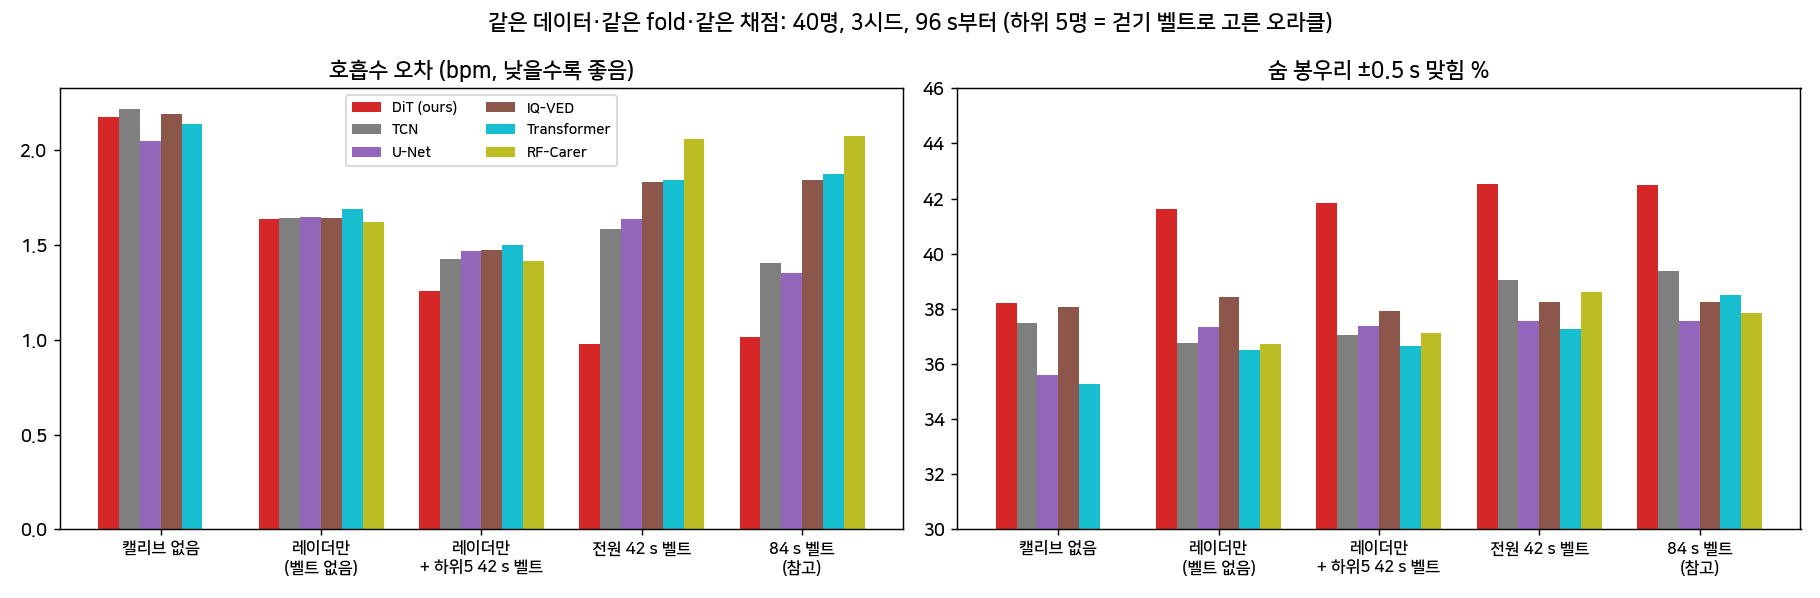
\includegraphics[width=\linewidth]{compare.png}
  \caption{캘리브레이션 단계별 DiT와 비교 모델의 호흡수 오차(왼쪽)와 숨 봉우리 일치율(오른쪽).}
  \label{fig:compare}
\end{figure}

\begin{figure}[t]
  \centering
  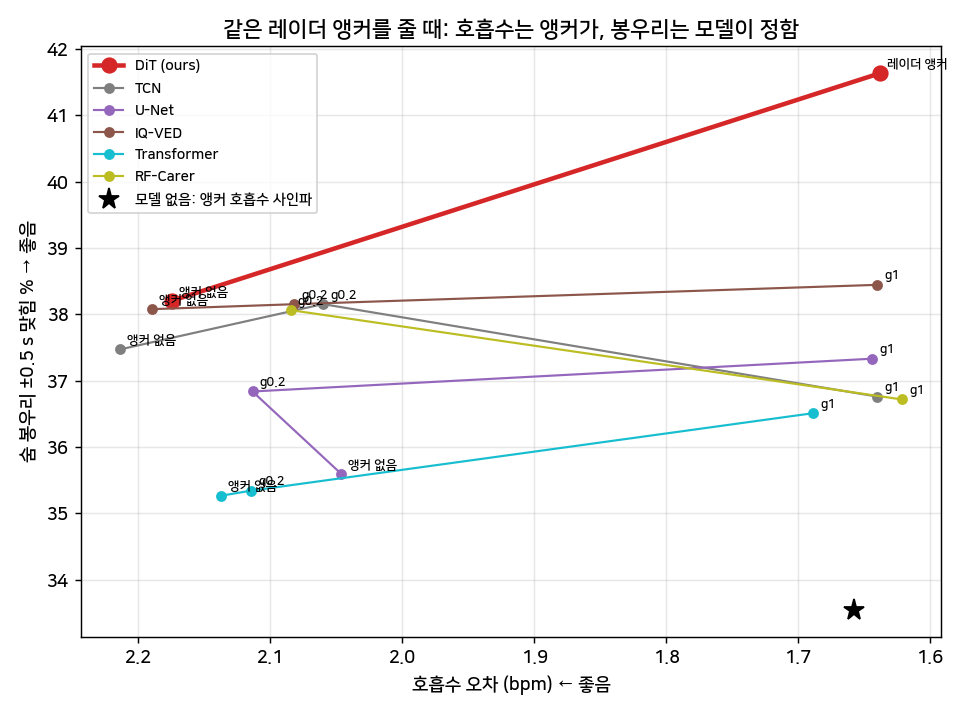
\includegraphics[width=0.62\linewidth]{tradeoff.png}
  \caption{같은 레이더 호흡수 앵커를 적용할 때의 호흡수 오차--봉우리 일치율 관계. 별표는 모델 없이 앵커 호흡수의 사인파를 출력한 경우이다.}
  \label{fig:tradeoff}
\end{figure}

\subsection{이중 레이더의 효과}
레이더 앵커 구성에서 레이더를 한 대만 사용하도록 학습한 모델과 비교하면, 두 대를 사용한 모델의 봉우리 일치율이 COM 단독 대비 7.1\%p($p{=}.0001$), TV 단독 대비 5.7\%p($p{=}.004$) 높았고
골 일치율도 각각 5.4\%p, 4.8\%p 높았다. 호흡수 앵커를 동일하게 고정한 경우에도 봉우리 일치율 차이는 4.1\%p($p{=}.006$), 4.8\%p($p{=}.02$)로 유지되어,
두 번째 레이더의 이득이 앵커 차이가 아닌 파형 타이밍에서 나온다는 것을 확인하였다.

\subsection{위치 추정과 호흡수 조절 가능성}
DiT의 구역 헤드는 14개 구역(우연 수준 7.1\%)에서 92.9\%의 정확도를 보였다.
또한 호흡수 앵커를 $\pm$3~bpm 바꾸었을 때 출력 호흡수가 평균 62\% 비율로 따라 움직여(40명 모두 같은 방향, $p<10^{-7}$),
호흡수 변화가 다른 경로(예: 정지 구간 측정)로 주어지면 이를 반영할 수 있음을 확인하였다.

%==============================================================
\section{논의 및 한계}
%==============================================================
결과는 17~fps 보행 조건에서 레이더와 캘리브레이션의 역할이 분리됨을 보여 준다.
호흡수 수준은 주로 캘리브레이션 앵커가 결정하며, 레이더 신호는 숨의 시점(타이밍)을 맞추는 데 기여한다.
따라서 개인 호흡수를 더 정확히 추정할 수 있는 단서가 확보될수록 성능이 직접 향상될 것으로 기대된다.

본 연구의 한계는 다음과 같다. 첫째, 정해진 경로와 일정한 구역 전환 리듬을 가진 보행 프로토콜에서 수집된 단일 데이터셋으로 평가하였다.
둘째, 전처리 단계는 현재 오프라인으로 수행되며 실시간 처리는 모델 추론 시간만 측정하였다.
셋째, 레이더만의 캘리브레이션에서 호흡수가 집단 평균과 크게 다른 사람의 오차가 크다.
향후에는 레이더 관측을 측정 모델로 명시하고 확산 모델의 사전분포와 결합하는 역문제 관점의 복원으로 확장하고, 자유 보행과 다른 환경의 데이터로 검증할 계획이다.

%==============================================================
\section{결론}
%==============================================================
본 논문은 17~fps 저가 IR-UWB 레이더 두 대를 ㄱ자 경로에 이중 각도로 배치하고, 레이더 기반 단서와 코스 리듬, 짧은 벨트 등록을 단계적으로 결합하는 캘리브레이션과
다중 작업 조건부 확산 트랜스포머를 이용하여 보행 중 호흡 파형과 실내 위치를 함께 추정하는 방법을 제안하였다.
피험자 40명에 대한 실험에서 벨트 없이 호흡수 오차 1.64~bpm, 42~s 등록으로 0.97~bpm을 달성하였으며, 동일 조건의 회귀 기반 모델 5종보다 숨 타이밍을 일관되게 더 잘 복원하였다.

\end{document}
